\documentclass[tikz,border=10pt]{standalone}
\begin{document}
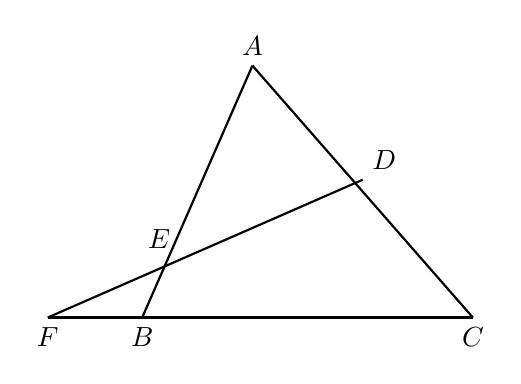
\begin{tikzpicture}
  \coordinate (A) at (2.6,3.2);
  \coordinate (B) at (1.2,0);
  \coordinate (C) at (5.4,0);
  \coordinate (F) at (0,0);
  \coordinate (D) at (4.0,1.75);
  \coordinate (E) at (1.68,1.0);

  \draw[thick] (F) -- (C);
  \draw[thick] (A) -- (C);
  \draw[thick] (A) -- (B);
  \draw[thick] (F) -- (D);

  \node[above] at (A) {$A$};
  \node[below] at (B) {$B$};
  \node[below] at (C) {$C$};
  \node[below] at (F) {$F$};
  \node[above right] at (D) {$D$};
  \node[left] at (E) {$E$};
\end{tikzpicture}
\end{document}
